\documentclass{article}

\usepackage[letterpaper, portrait, margin=1.5in]{geometry}

\usepackage{fancyhdr}
\usepackage{ragged2e}
\usepackage{graphicx}
\usepackage{caption}
\usepackage{amsmath}
\usepackage{rotating}

\usepackage{listings}
\usepackage{color}

\definecolor{dkgreen}{rgb}{0,0.6,0}
\definecolor{gray}{rgb}{0.5,0.5,0.5}
\definecolor{mauve}{rgb}{0.58,0,0.82}

\lstset{frame=tb,
  language=Java,
  aboveskip=3mm,
  belowskip=3mm,
  showstringspaces=false,
  columns=flexible,
  basicstyle={\small\ttfamily},
  numbers=none,
  numberstyle=\tiny\color{gray},
  keywordstyle=\color{blue},
  commentstyle=\color{dkgreen},
  stringstyle=\color{mauve},
  breaklines=true,
  breakatwhitespace=true,
  tabsize=4
}

\setcounter{secnumdepth}{1}

\usepackage{chngcntr}
\counterwithin{figure}{section}

\renewcommand*{\thepage}{C\arabic{page}}

\pagestyle{fancy}
\lhead{ACME Robotics}
\chead{\#8367}
\rhead{\ifcontents Contents \else Week \thesection \fi}

\newif\ifcontents
\contentstrue

\makeatletter
\renewcommand{\@seccntformat}[1]{}
\makeatother
\begin{document}

\subsubsection{Re-tune lift}
%! its exactly what it sounds like
Now that the new lift was on the robot, Kelly decided it was time to re-tune the lift. Because there is only one encoder between the two lift motors, it is not safe to use \texttt{RUN\_USING\_ENCODERS}, so the control loop needs a normal tuning, with $k_v$, $k_a$, and $k_{static}$. Kelly began by writing an opmode to gradualy ramp up the voltage applied to the lift motors until the lift reached either the top or the bottom, then stop the lift and revers. The opmode logged both the applied power and the actual velocity of the lift in a csv file, and because the lift was accelerating so gradualy it was safe to assume that the only acceleration on the lift was due to gravity. After running the opmode for a while and collecting a lot of data, Kelly pulled the file off the phones, and seperated them using a python script based on the direction the lift was moving, and the state of the sensor that detected the frame being at the bottom of its range of motion. The data from the lift moving down while the frame was at the bottom was super noisy, so Kelly threw it out and only considered the other three sets. The graph in figure \ref{fig:liftData} shows the collected data. As you can see, the slope of all three groups of data is the same, but the intercept is different. 

Because the neccecary voltage to achieve a particular motion state in a linear mechanism is $$V = \omega k_v + \alpha k_a + k_static$$ 
and the acceleration across all the runs is constant (gravitational acceleration, $386 in/sec^2$, the slope of all the graps is $\frac{1}{k_v}$, and the intercept is a combination of $k_a$ and $k_{static}$. Because $k_a$ is dependent on the mass of the thing that is moving (and in fact can be written as $k_a = m k_f$), it is important to compare lines with constant mass when calculating $k_static$. By comparing both states where both the carriage and the frame are moving (when the mass of the parts of the lift that are in motion are greatest), (shown in purple and blue in figure \ref{fig:liftData} $k_{static}$ and $k_a$ (for that mass, and by extension $k_f$) can be calculated. Because $k_a$ is going to be the same for both, and $k_{static}$ is going to have the same magnitude but opposite signs (because its sign is the same as the direction of travel), $k_a$ was found to be the midpoint between the two intercepts, and $k_static$ is one half of the distance between them. By dividing the calculated $k_a$ by the mass of the entire lift, Kelly found $k_f$. 

The following listing shows the way a feedforward command is actualy calculated from a desired motion state and known mass.
\begin{lstlisting}[language=Java]
    public static double K_V = 0.0643202688898;
    public static double K_STATIC = 0.118777073737;
    public static double K_A = 0.000127390384279;
    public static double MASS_ROBOT = -20;
    public static double MASS_CARTRIGE = .75;
    public static double MASS_FRAME = .75;
    public static double G = 386;

    private double getFeedForward (MotionState state, double mass) {
        double ff = K_V * state.getV() + K_A * mass * (state.getA() - G);
        if (Math.abs(ff) > 1e-4) ff +=  Math.copySign(K_STATIC, ff);
        return ff;
    }
\end{lstlisting}

\begin{figure}
    \centering
    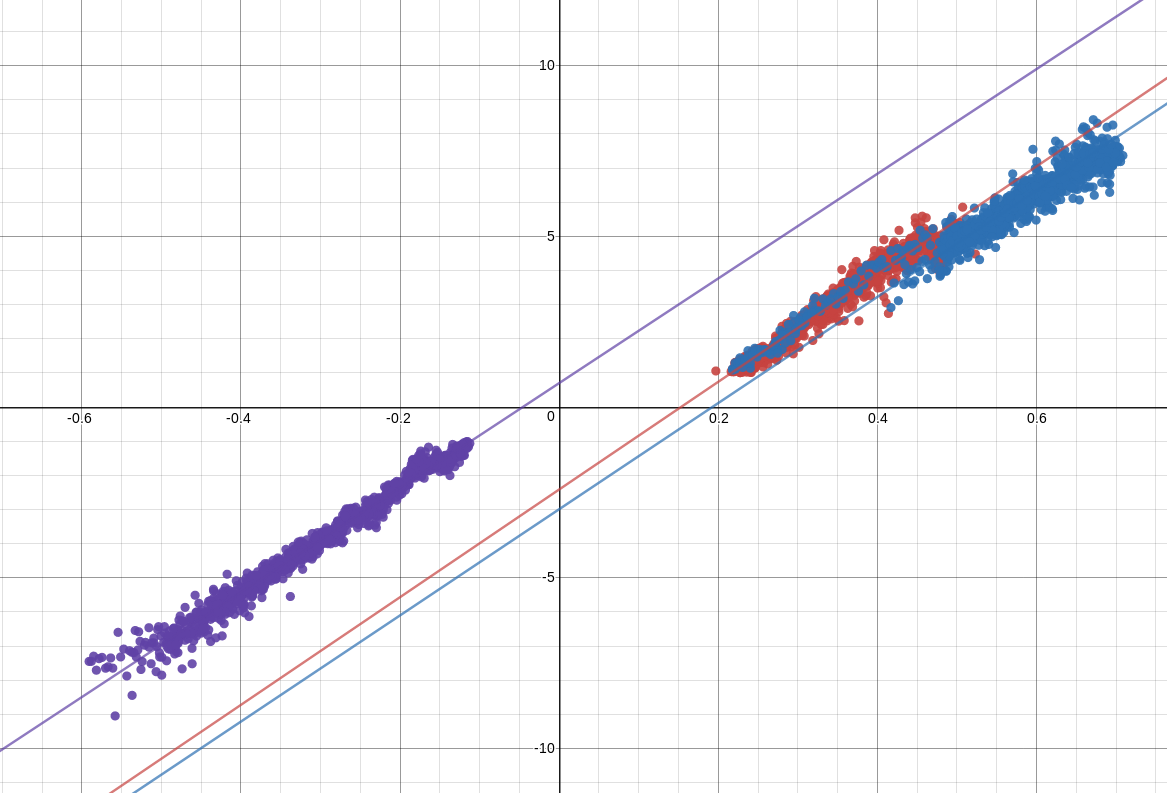
\includegraphics[width=.6\textwidth]{30_03-25/images/graph.png}
    \caption{Collected lift data}
    \label{fig:liftData}
\end{figure}

This listing shows the way this function is used within the profile following code.
\begin{lstlisting}
        MotionState target = profile.get(t);
        double error = getPosition() - target.getX();
        double correction = pidController.update(error);
        double feedForward = getFeedForward(target, getMass());
        internalSetVelocity(feedForward - correction);
\end{lstlisting}


\end{document}